\documentclass{article}
\usepackage{graphicx} % Required for inserting images
\renewcommand*\thetable{\Roman{table}}
\usepackage[a4paper, total={6in, 10in}]{geometry}
\usepackage{titlesec}
\usepackage{hyperref}
\hypersetup{
    colorlinks=true,
    linkcolor=blue,
    filecolor=magenta,      
    urlcolor=blue,
    pdftitle={Overleaf Example},
    pdfpagemode=FullScreen,
    }
    
\titlespacing\section{0pt}{12pt plus 4pt minus 2pt}{10pt plus 2pt minus 2pt}
\titlespacing\subsection{0pt}{12pt plus 4pt minus 2pt}{8pt plus 2pt minus 2pt}
\title{Electron Trajectory}
\author{Alex Benitez}
\date{25 February 2024}

\begin{document}
\maketitle
\section*{Generating trajectories}
After reading through the Thomas Siegel thesis a couple of times, I came to grips first with the intuitive side of the three step model, and later the mathematics. Afterwards, my task was to program the trajectory of the electron after it leaves the atomic potential, initially I tried to do this with seaborne, in order to learn a new skill and make some pretty graphs, but eventually realized it wasn't as well suited to the types of plots I wanted to make as good old matplotlib, so I settled for that instead. After a couple of attempts at inserting the formula found in the thesis:
\begin{equation}
    x(t) = \frac{-e}{m \omega^2_0}\left[E_0(t)cos(\omega_0 t + \phi) - E_0(t_i)cos(w_0 t_i + \phi) \right] - \frac{-e E_0 (t_i}{m \omega^2_0} (t - t_i) sin( \omega_0 t + \phi)
\end{equation}

After some attempting and tinkering, I did not manage to implement the formula, and still have a couple of doubts as to the terms, so instead I used the traditional equations of motion, which yielded much better results:
\begin{figure}[h!btp]
\centering

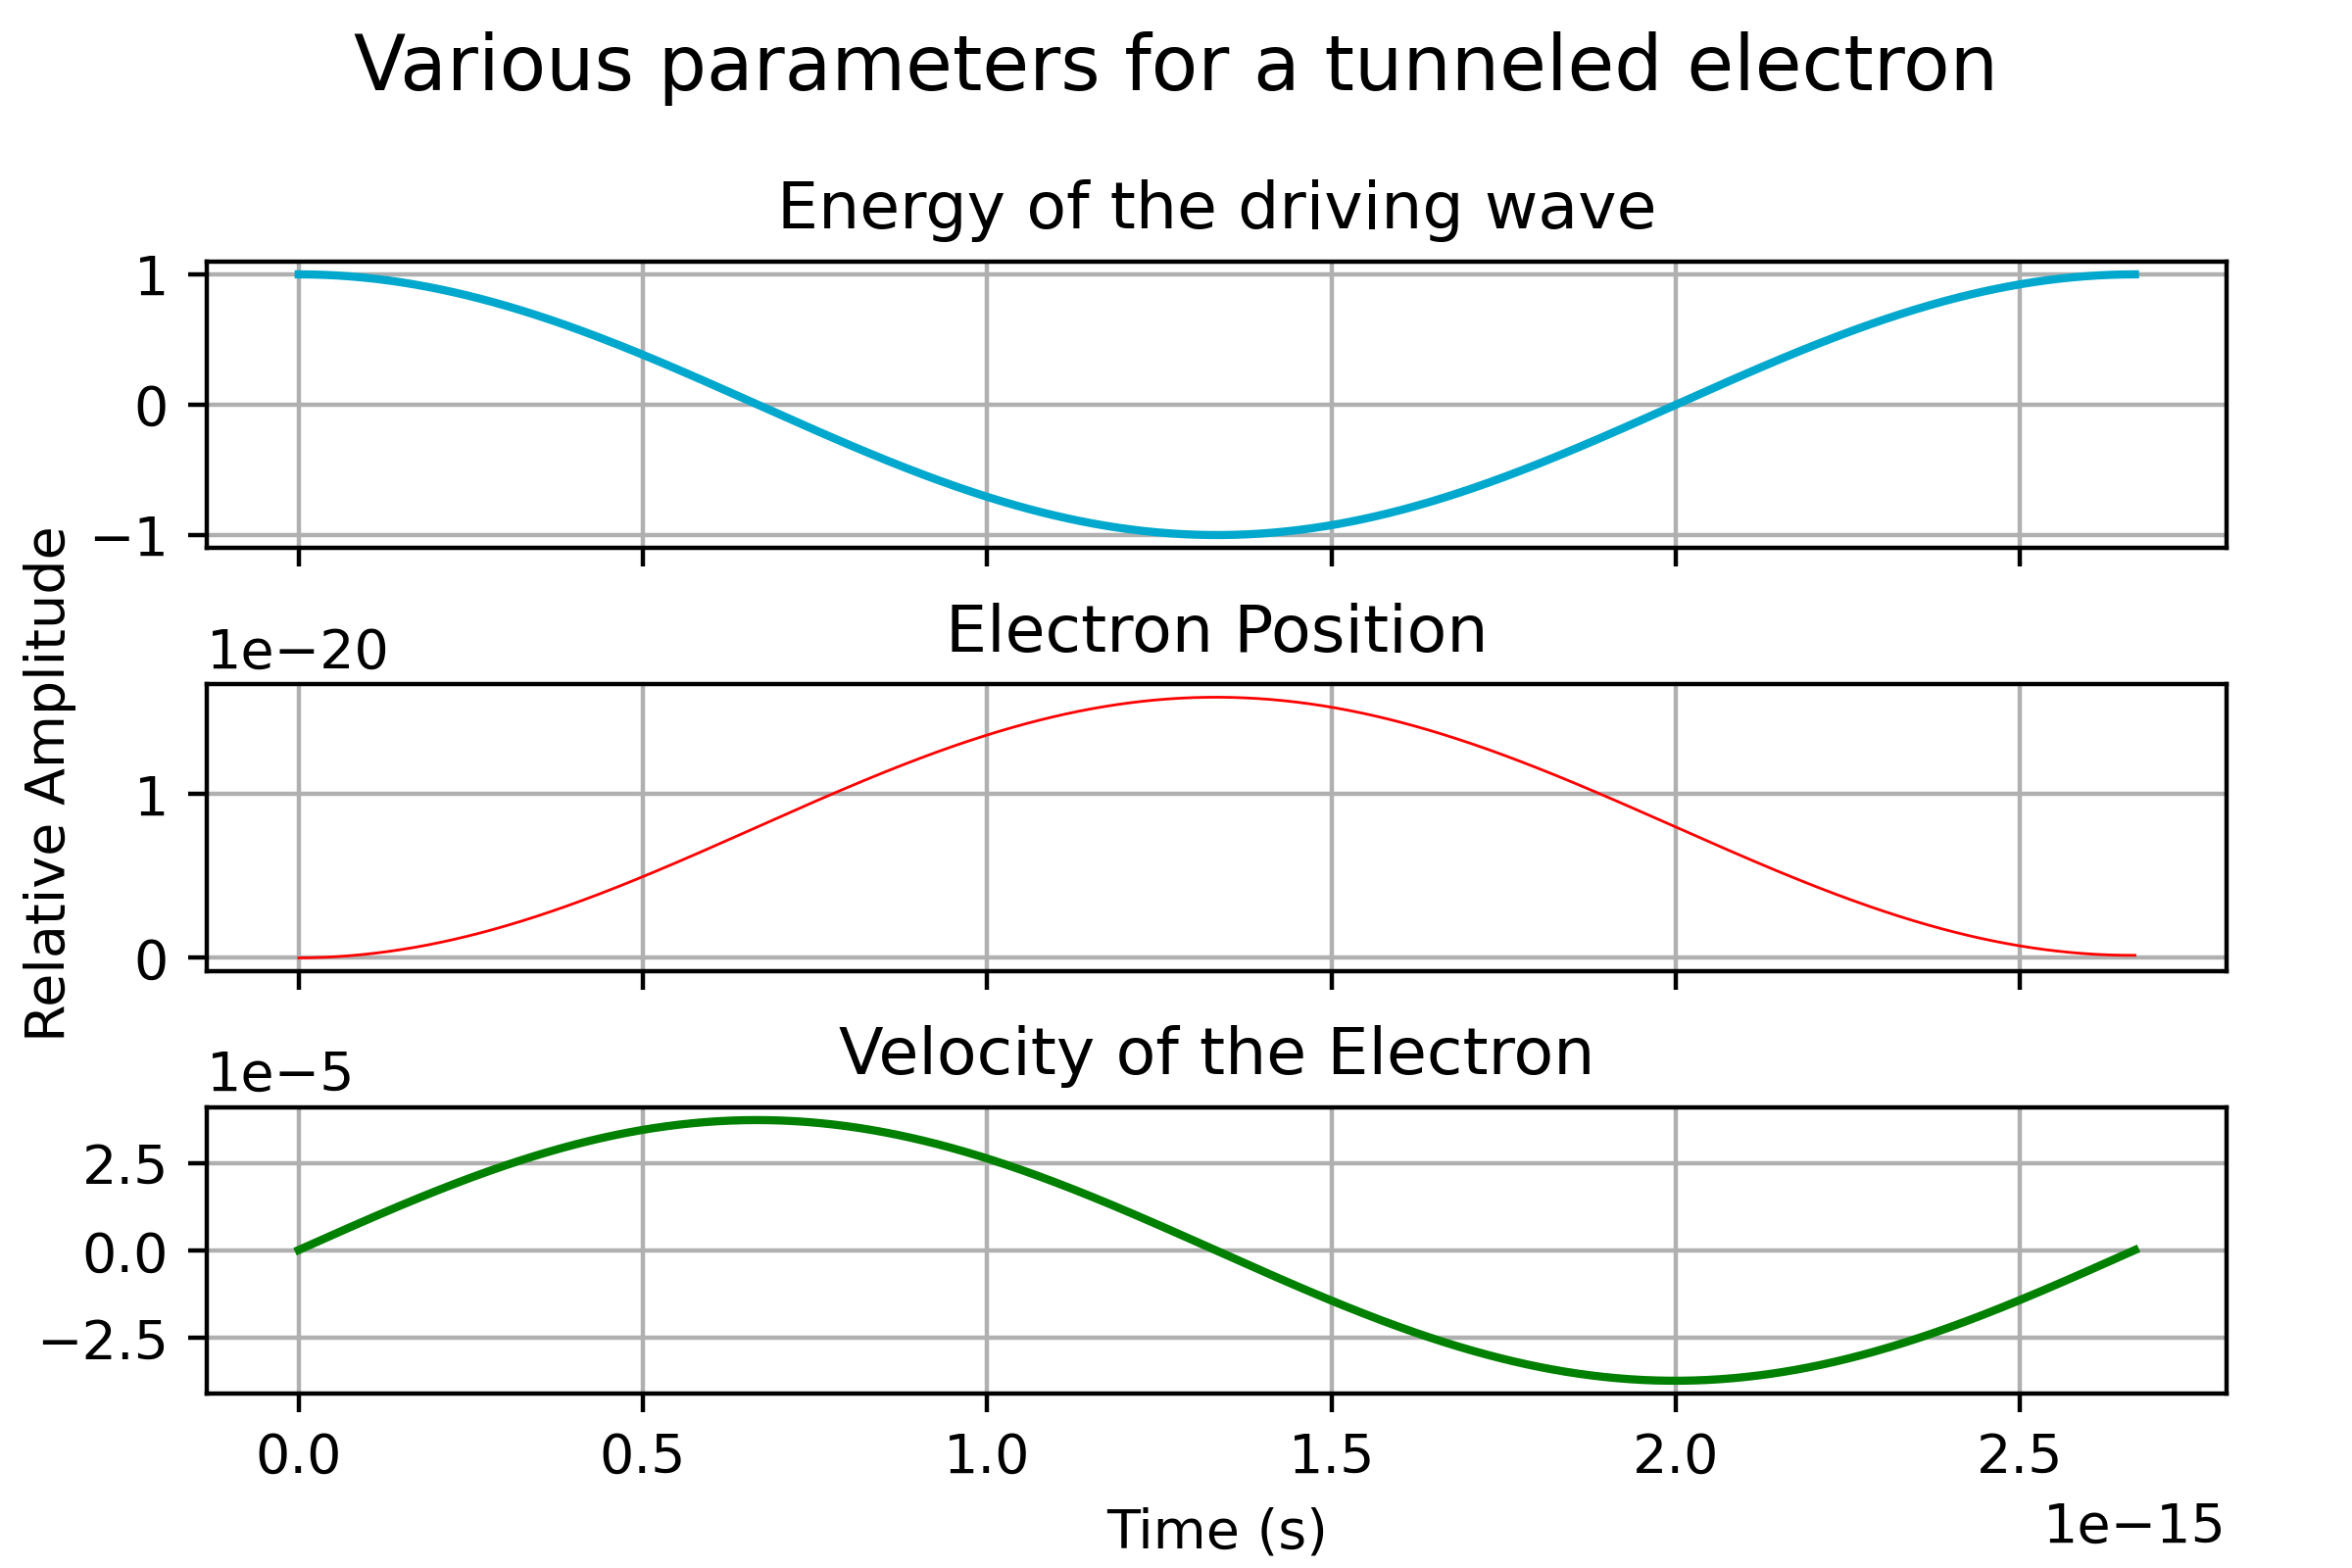
\includegraphics[width=0.95\linewidth]{electrontraj.png}
\textbf{\caption{Pretty (and) self explanatory graph}}
\centering
\end{figure}

Satisfied with this graph, which accurately (I think) describes the motion of the electron and the velocity. I also created a github repository to keep track of the code (and for postgrad/employers of course) which is linked here:
\url{https://github.com/alex-benitez/Atto}

\pagebreak

Additionally you can add phase to the trajectory, and get a slightly different graph:
\begin{figure}[h!btp]
\centering

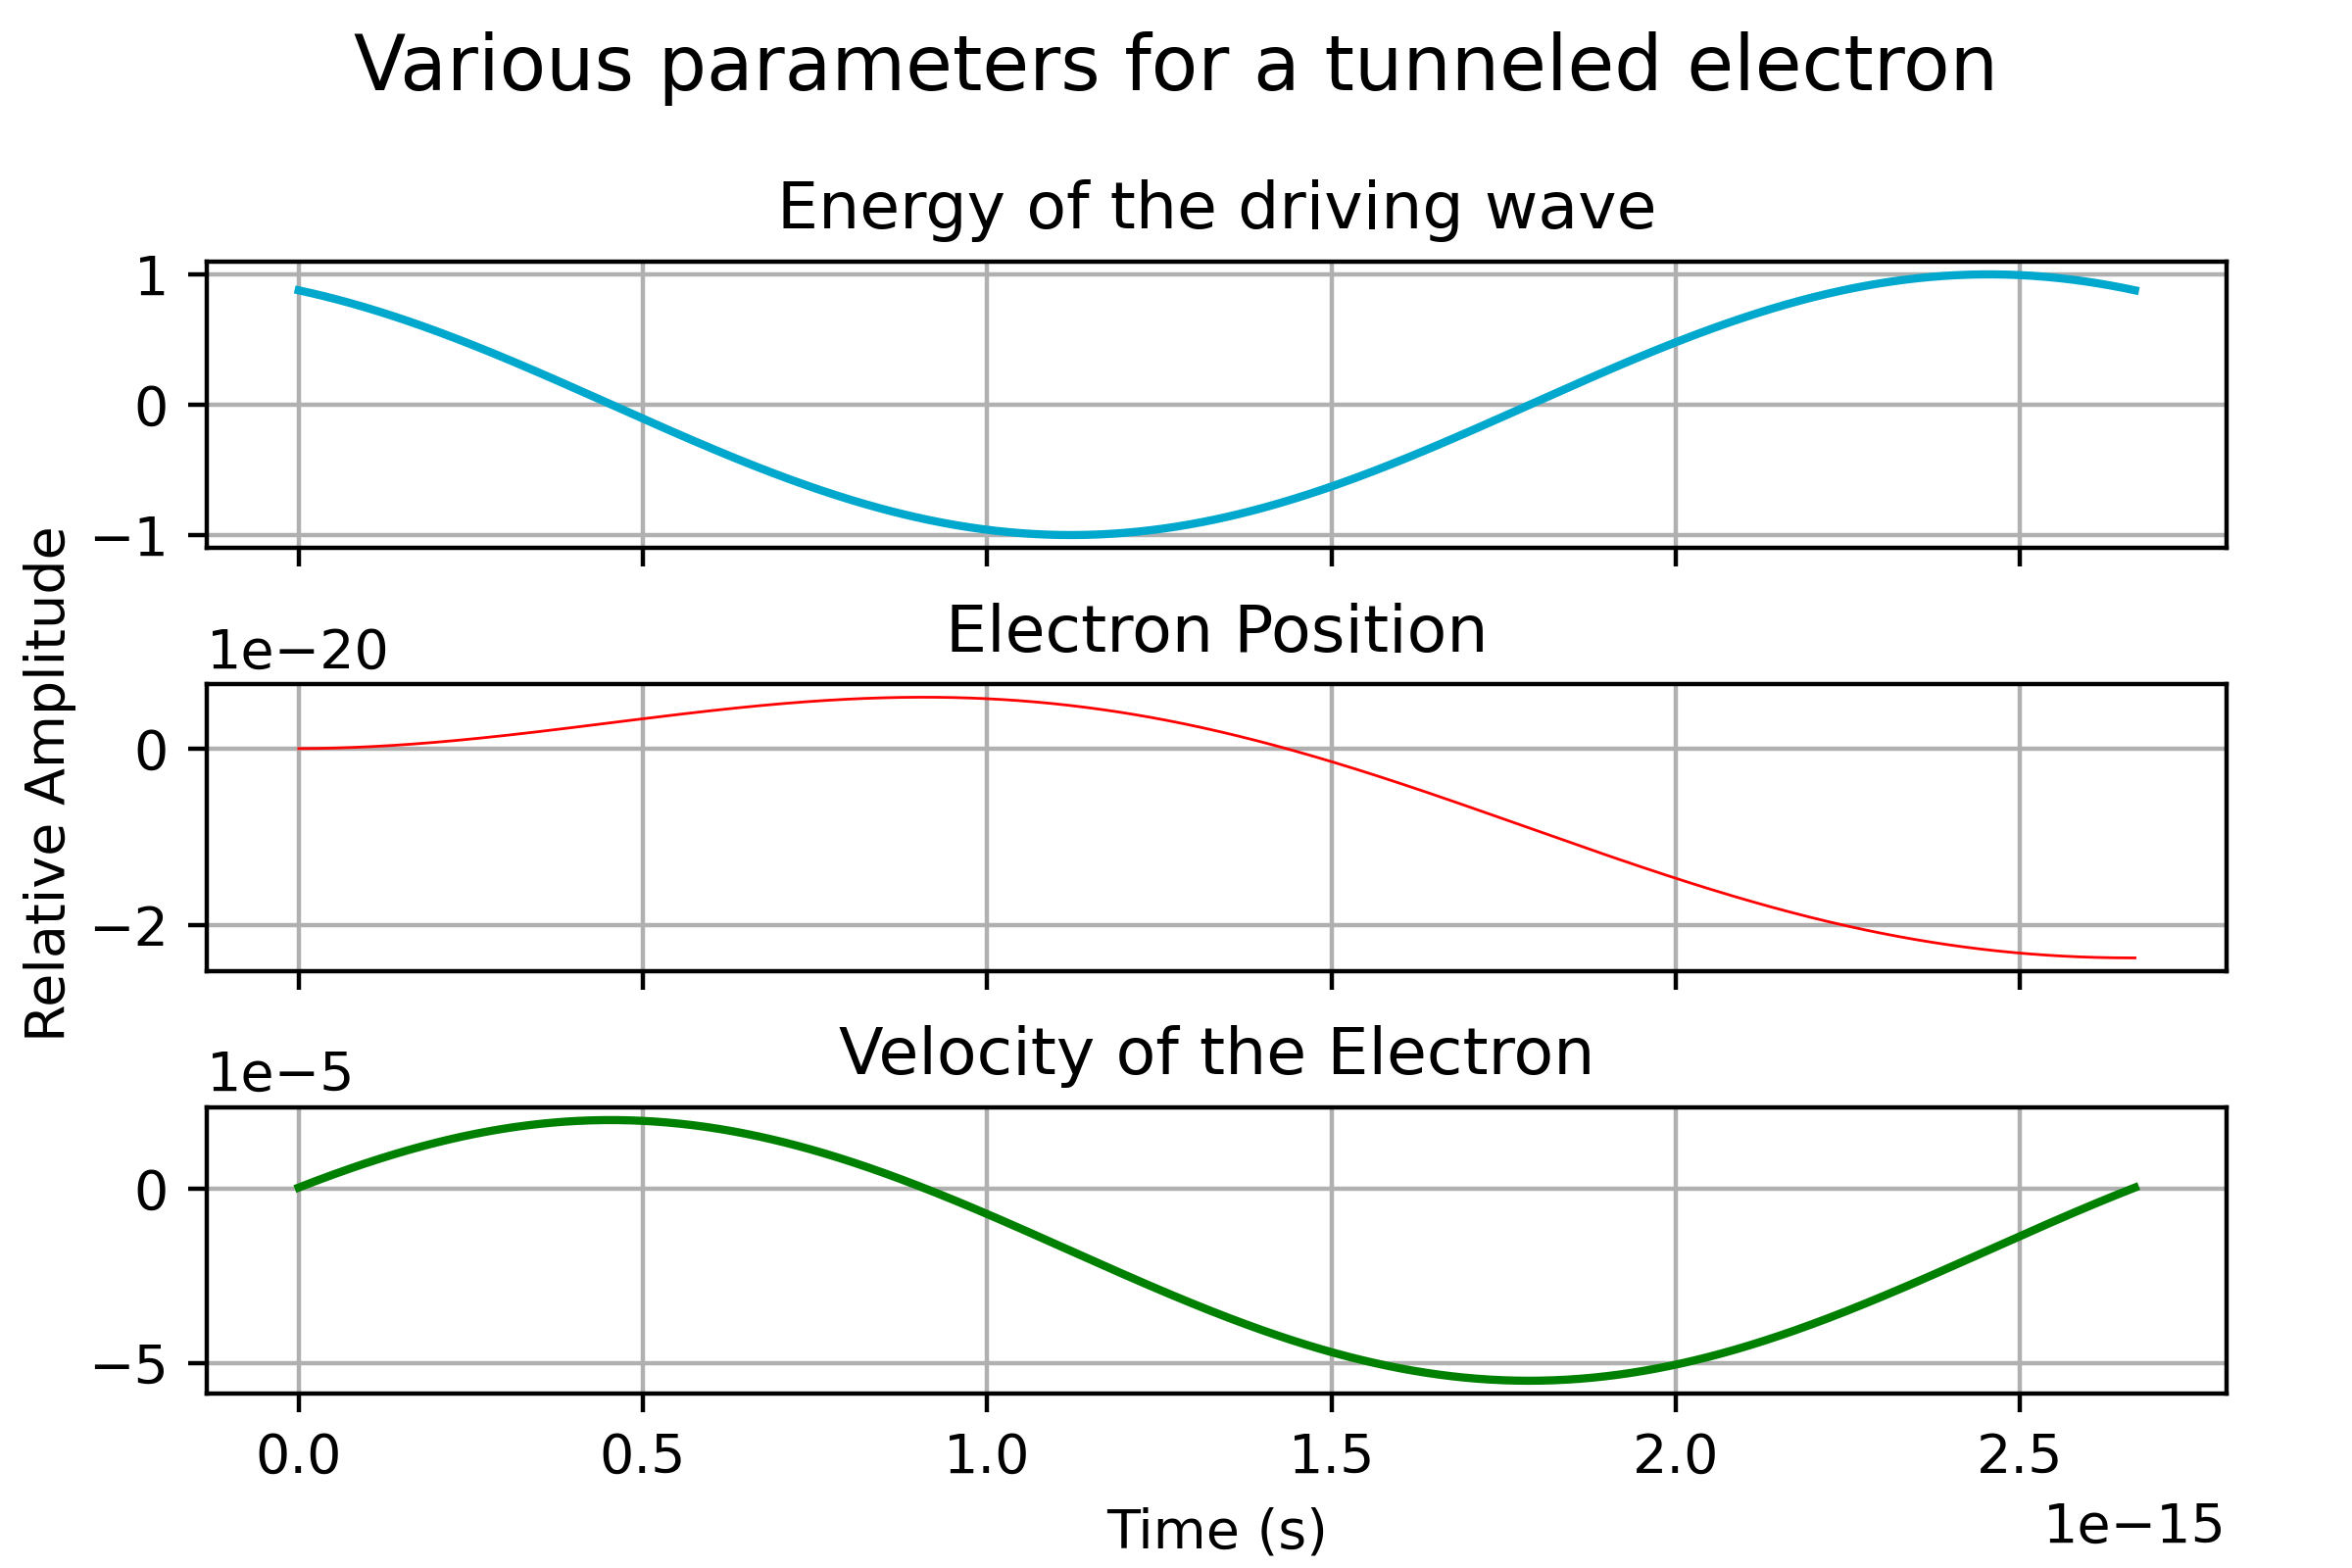
\includegraphics[width=0.95\linewidth]{electrontrajphase.png}
\textbf{\caption{Added phase of 0.5 radians}}
\centering
\end{figure}

The next logical step is to create a distribution of electrons exiting the nucleus at a given phase, and use that to plot the graph of possible positions.


\end{document}
